\chapter{Pendahuluan}

\section{Sejarah Pemrograman dan Python}

Pemrograman komputer dimulai pada abad ke-19 dengan penemuan mesin analitik oleh Charles Babbage dan program pertama yang ditulis oleh Ada Lovelace. Sejak itu, pemrograman telah berkembang pesat dengan munculnya bahasa-bahasa pemrograman awal seperti Fortran, COBOL, dan Lisp pada tahun 1950-an. Pada tahun 1970-an dan 1980-an, bahasa pemrograman seperti C, Pascal, dan Basic memperkenalkan konsep-konsep baru dalam pemrograman. Kini, berbagai bahasa pemrograman modern seperti Python, JavaScript, dan Rust digunakan dalam berbagai aplikasi.

Python merupakan bahasa pemrograman \textit{high-level} serbaguna yang pertama kali diperkenalkan pada tahun 1991 oleh Guido van Rossum (GvR). Bahasa ini dirancang agar mudah dipahami dan memiliki struktur kode yang jelas (\textit{readable}), serta mendukung fitur penanganan kesalahan (\textit{exception handling}). Dengan tujuan tersebut, Python berhasil berkembang menjadi bahasa pemrograman yang dapat dimanfaatkan di berbagai bidang. Python merupakan bahasa pemrograman multi-paradigma, yang artinya dapat menggunakan gaya/metode beragam dalam penulisan kode. Saat ini, Python banyak digunakan untuk pengembangan aplikasi web (\textit{server-side}), analisis data, hingga penerapan kecerdasan buatan dan pembelajaran mesin (\textit{machine learning}).

\section{Python Sebagai Bahasa Interpreter}
Python merupakan bahasa pemrograman yang termasuk ke dalam kategori
\textit{interpreted language}. Artinya, kode program Python tidak
dikompilasi terlebih dahulu menjadi file biner yang dapat dieksekusi,
melainkan dijalankan baris demi baris oleh sebuah program bernama
\textbf{interpreter}.

Interpreter bertugas membaca kode Python, menerjemahkannya, lalu
menjalankannya secara langsung. Hal ini membuat proses pengembangan
program menggunakan Python menjadi lebih fleksibel, karena kita bisa
langsung menuliskan kode dan melihat hasil eksekusinya tanpa melalui
tahap kompilasi.

\begin{figure}[H]
	\centering
	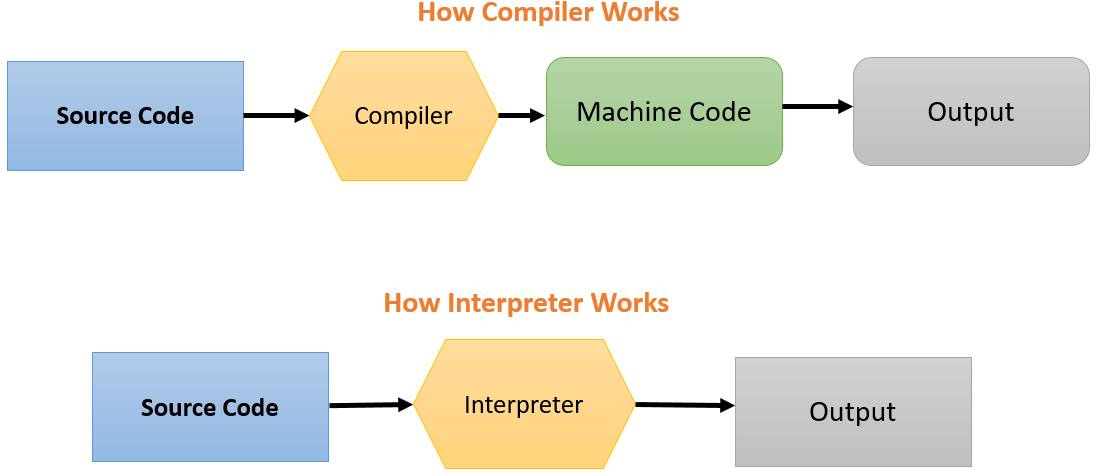
\includegraphics[width=0.7\textwidth]{../shared_assets/images/compiler_vs_interpreter.png}
	\caption{Perbedaan antara Compiler dan Interpreter}
	\label{fig:compiler-vs-interpreter}
\end{figure}

\noindent
Pada Gambar \ref{fig:compiler-vs-interpreter} dapat dilihat perbedaan
utama antara \textit{compiler} dan \textit{interpreter}.  
\begin{itemize}
	\item \textbf{Compiler}: Menerjemahkan seluruh kode sumber menjadi file biner terlebih dahulu, kemudian hasilnya dapat dijalankan berulang kali tanpa perlu proses kompilasi ulang.
	\item \textbf{Interpreter}: Menjalankan kode baris demi baris secara langsung, sehingga lebih mudah untuk debugging dan eksplorasi.
\end{itemize}

\noindent
\textbf{Kelebihan Python sebagai bahasa interpreter:}
\begin{enumerate}
	\item Mudah digunakan untuk pemula karena tidak perlu memahami proses kompilasi.
	\item Memungkinkan interaksi langsung melalui \textit{interactive shell}.
	\item Sangat fleksibel untuk \textit{prototyping} dan eksperimen cepat.
\end{enumerate}

\noindent
\textbf{Kekurangan Python sebagai bahasa interpreter:}
\begin{enumerate}
	\item Lebih lambat dibandingkan bahasa yang dikompilasi murni (seperti C, C++, atau Java).
	\item Program Python membutuhkan interpreter terpasang di sistem agar bisa dijalankan.
\end{enumerate}

\noindent
Sumber gambar: \url{https://www.ankitweblogic.com/c/compiler-and-interpreter.php}

\section{Instalasi di Windows}
Untuk menginstal Python di Windows, ikuti langkah-langkah berikut:

\begin{enumerate}
\item Unduh installer Python terbaru dari situs resmi \href{https://www.python.org/downloads/}{python.org}.
\item Jalankan file installer \texttt{.exe} dan ikuti petunjuk untuk menyelesaikan instalasi.
\item Saat instalasi, centang opsi \textbf{``Add Python to PATH''} agar Python otomatis dikenali di Command Prompt.
\item Ikuti petunjuk instalasi hingga selesai.
\item Verifikasi instalasi dengan membuka Command Prompt lalu ketik:
\begin{verbatim}
    python --version
    pip --version
\end{verbatim}
\end{enumerate}

\section{Instalasi di macOS}

Untuk menginstal Python di macOS, ikuti langkah-langkah berikut:

\begin{enumerate}
\item Unduh installer Python terbaru dari \href{https://www.python.org/downloads/macos/}{python.org}.
\item Jalankan file installer \texttt{.pkg} dan ikuti petunjuk hingga selesai.
\item Alternatif lain, Anda bisa menggunakan Homebrew dengan menjalankan perintah berikut di Terminal:
\begin{verbatim}
    brew install python
\end{verbatim}
\item Setelah instalasi selesai, verifikasi dengan perintah:
\begin{verbatim}
    python3 --version
    pip3 --version
\end{verbatim}
\end{enumerate}

\section{Instalasi di Linux}

Untuk menginstal Python di Linux, ikuti langkah-langkah berikut:

\begin{enumerate}
\item Buka terminal dan jalankan perintah berikut untuk memastikan repositori diperbarui dan Python terpasang:
\begin{verbatim}
    sudo apt update
    sudo apt install python3 python3-pip
\end{verbatim}
\item Verifikasi instalasi dengan perintah:
\begin{verbatim}
    python3 --version
    pip3 --version
\end{verbatim}
\end{enumerate}

\section{IDE dan Editor untuk Python}

\subsection{Apa Itu IDE?}

Integrated Development Environment (IDE) adalah perangkat lunak yang menyediakan fasilitas lengkap untuk pengembangan perangkat lunak. IDE umumnya mencakup editor kode, kompiler atau interpreter, debugger, dan alat manajemen proyek. IDE dirancang untuk mempermudah proses pengembangan perangkat lunak dengan menyediakan antarmuka pengguna yang terintegrasi dan alat-alat yang mendukung pengkodean, pengujian, dan debugging.

Dalam praktikum Python, terdapat beberapa pilihan IDE atau editor yang bisa digunakan, antara lain Visual Studio Code, IDLE (editor bawaan Python), dan PyCharm. Namun, Anda dapat menggunakan IDE atau editor lain yang Anda sukai. Modul praktikum ini menggunakan Visual Studio Code sebagai contoh.

\subsection{Cara Menginstal Visual Studio Code}

\begin{enumerate}
    \item Unduh installer VS Code dari situs resmi \url{https://code.visualstudio.com/}.
    \item Pilih installer sesuai sistem operasi Anda (Windows, macOS, atau Linux).
    \item Jalankan file installer dan ikuti petunjuk instalasi.
    \item Setelah instalasi selesai, buka aplikasi VS Code.
    \item Untuk mendukung pemrograman Python, instal ekstensi \textbf{Python} dari Microsoft melalui menu Extensions (ikon kotak di sidebar kiri).
    \item Untuk membuat file Python, buka menu File (ikon kotak di sidebar kiri) lalu pilih New File (ikon kotak di sidebar kiri) dan ketik nama file yang diinginkan diakhiri dengan \texttt{.py}. Contoh \texttt{hello.py}.
    \item Sekarang Anda dapat mulai menulis dan menjalankan kode Python di dalam VS Code.
\end{enumerate}

\section{Kode Python: hello_world.py}
\label{sec:hello-world-code}

\begin{lstlisting}[style=PythonStyle, caption={Kode Python: hello_world.py}]
print("Hello World!")
\end{lstlisting}

Kode di atas merupakan program Python sederhana yang mencetak "Hello World!" ke konsol. Berikut penjelasan dari setiap bagian kode tersebut:

\begin{itemize}
\item \texttt{print(...)} – \texttt{print} adalah fungsi bawaan (\textit{built-in function}) di Python yang digunakan untuk menampilkan output ke layar atau konsol.
\item \texttt{"Hello World!"} – Merupakan sebuah string (teks) yang ditulis di dalam tanda kutip ganda. Nilai string ini akan menjadi argumen yang dikirim ke fungsi \texttt{print}.
\end{itemize}

\section{Panduan Menjalankan Program Python}

Untuk menjalankan program Python di atas, ikuti langkah-langkah berikut:

\begin{enumerate}
	\item Buka terminal atau command prompt.
	\item Navigasikan ke direktori tempat file `hello_world.py` disimpan.
	\begin{verbatim}
		cd /path/ke/direktori
	\end{verbatim}
	\item Jalankan perintah berikut untuk mengkompilasi program:
	\begin{verbatim}
		python hello_world.py
	\end{verbatim}
	\item Jika tidak ada error, program akan dijalankan dan menampilkan "Hello World!" di konsol.
\end{enumerate}

\section{Kode Python: hello_with_input.py}

\begin{lstlisting}[style=PythonStyle, caption={Kode Python: hello_with_input.py}]
nama = input("Masukkan nama Anda: ") # Menerima input dari pengguna

print("Hello " + nama + "!") # Menampilkan output dengan input pengguna
\end{lstlisting}

Berikut penjelasan dari setiap bagian kode tersebut:

\begin{itemize}
\item \texttt{nama = input("Masukkan nama Anda: ")} - Fungsi input merupakan \textit{built-in function} yang digunakan untuk menerima input pengguna dari konsol. Fungsi ini menunda eksekusi program sampai pengguna memasukkan input dan menampilkan opsional pesan untuk meminta input yang kemudian disimpan dalam variabel \texttt{nama}.
\item \texttt{print("Hello " + nama + " !")} - Seperti yang dijelaskan pada Section~\ref{sec:hello-world-code}, fungsi print digunakan untuk mencetak output ke layar atau konsol. Di sini, pesan "Hello [Nama]!" diisi dengan input pengguna.
\end{itemize}


\section{Latihan}

Berikut adalah beberapa latihan yang dapat Anda coba untuk memperdalam pemahaman tentang program Python yang telah dibahas:

\begin{enumerate}
\item \label{sec:first-exercise} \textbf{Latihan 1:} Buat file baru dengan nama \textbf{introduction.py} yang dimana program harus menerima input nama, program studi, dan tahun angkatan dari pengguna kemudian mencetak pesan dengan format yang ditentukan
\begin{lstlisting}[style=PythonStyle, caption={Latihan 1}]
nama = input("Masukkan nama Anda: ")
prodi = input("Masukkan program studi Anda: ")
angkatan = input("Masukkan tahun angkatan Anda: ")

print("Halo! Nama saya " + nama + ". Saya mahasiswa program studi " + prodi + " tahun angkatan " + angkatan + ".")
\end{lstlisting}

Contoh input dan output yang diberikan ketika program dijalankan:

\begin{verbatim}
Input:
Masukkan Nama Anda: Bob Smith
Masukkan Program Studi Anda: Informatika
Masukkan Tahun Angkatan: 2025

Output:
Halo! Nama saya Bob Smith. Saya mahasiswa program studi Informatika tahun angkatan 2025.
\end{verbatim}

\item \textbf{Latihan 2:} Latihan ini bertujuan untuk belajar memformat teks (\textit{string}) menggunakan \textbf{f-string}, membuat output lebih rapi tanpa perlu menggunakan operator \texttt{+} sebagai penghubung antara teks. Buat file baru dengan nama \textbf{introduction_with_fstring.py} dan isinya mirip dengan \hyperref[sec:first-exercise]{Latihan 1}, namun format outputnya menggunakan \textbf{f-string}

\begin{lstlisting}[style=PythonStyle, caption={Latihan 2}]
nama = input("Masukkan nama Anda: ")
prodi = input("Masukkan program studi Anda: ")
angkatan = input("Masukkan angkatan Anda: ")

print(f"Halo! Nama saya {nama}. Saya mahasiswa program studi {prodi} tahun angkatan {angkatan}. Output dihasilkan menggunakan f-string")
\end{lstlisting}

Contoh input dan output yang diberikan ketika program dijalankan:

\begin{verbatim}
Input:
Masukkan Nama Anda: Bob Smith
Masukkan Program Studi Anda: Informatika
Masukkan Tahun Angkatan: 2025

Output:
Halo! Nama saya Bob Smith. Saya mahasiswa program studi Informatika tahun angkatan 2025. 
Output dihasilkan menggunakan f-string
\end{verbatim}

\item \textbf{Latihan 3:} \textit{Escape Character} merupakan karakter khusus yang digunakan (biasanya diawali dengan \texttt{\textbackslash}) yang digunakan di dalam string untuk mengatur penataan teks atau menampilkan karakter spesial. Dengan escape character, kita bisa:

\begin{itemize}
    \item Membuat teks pindah baris: \texttt{\textbackslash n}
    \item Menambahkan tabulasi: \texttt{\textbackslash t}
    \item Menulis tanda kutip di dalam string: \texttt{\textbackslash "}
    \item Menampilkan backslash asli: \texttt{\textbackslash\textbackslash}
\end{itemize}

Buat file baru dengan nama \textbf{escape_character.py} dan isinya seperti berikut:

\begin{lstlisting}[style=PythonStyle, caption={Latihan 3}]
print("Hello\nWorld") # Membuat teks pindah baris
print("Hello\tWorld") # Menambahkan tabulasi
print("Hello \"World") # Menulis tanda kutip di dalam string
print("Hello \\ World") # Menampilkan backslash asli
\end{lstlisting}

Output yang akan dihasilkan dari program di atas adalah:

\begin{verbatim}
Hello
World
Hello	World
Hello "World
Hello \ World
\end{verbatim}
\end{enumerate}

\section{Soal Latihan}

Berikut adalah beberapa soal latihan tambahan untuk menguji pemahaman Anda mengenai konsep yang telah dipelajari:

\begin{enumerate}
\item \textbf{Soal 1:} Buat program bernama \texttt{biodata.py} yang meminta input berupa:
\begin{itemize}
	\item Nama lengkap
	\item Umur
	\item Hobi
\end{itemize}
	Cetak output dengan format berikut menggunakan \textbf{f-string}. Berikut merupakan contoh input dan output yang diharapkan:
\begin{verbatim}
Input:
Masukkan Nama Lengkap: Jane Hopkins
Masukkan Usia Anda: 20
Masukkan Hobi Anda: Ngoding

Output:
Halo, nama saya Jane Hopkins. Saya berusia 20 tahun dan hobi saya adalah Ngoding.
\end{verbatim}

\item \textbf{Soal 2:}  
Buat program bernama \texttt{quote.py} yang menampilkan kutipan favoritmu. Gunakan \textbf{escape character} untuk menampilkan tanda kutip di dalam string. Contoh output:

\begin{verbatim}
Input:
Masukkan kutipan favoritmu dari Albert Einstein: "Imagination is more important 
than knowledge."

Output:
Kata Albert Einstein: "Imagination is more important than knowledge."
\end{verbatim}

\item \textbf{Soal 3:} Buat program bernama \texttt{schedule.py} yang menampilkan jadwal kuliah. Gunakan \textbf{tabulasi} (\texttt{\textbackslash t}) untuk merapikan kolom. Contoh output:

\begin{tabular}{l l l}
    \textbf{Hari} & \textbf{Waktu} & \textbf{Mata Kuliah} \\
    Senin & 07.00 & Algoritma \\
    Selasa & 09.00 & Basis Data \\
    Selasa & 13.00 & Pemrograman Dasar \\
\end{tabular}
\end{enumerate}
